\chapter{Experiments on Synthetic Data}
In this chapter we cover what synthetic datasets are used and how they are constructed for evaluating the online kernel change point detection methods discussed in the previous chapter. All the results of the experiments are then presented in section \ref{eval}.

\section{Setup}
\label{experiments}
\subsection{Initialization}
An important factor for online change point methods is determining how to initialize the algorithm. Because we are running an unsupervised model for classifying change points, we do not spend time training the model or tuning any of the hyperparameters. This is a double-edged sword because on one hand, we can drop in a change point algorithm onto a data stream and let it start running without much interference. On the other hand, if it does not have any prior distribution to compare to then it will need to be adjusted to know what's an appropriate reference or in-control distribution. This is usually referred to as the initialization phase for online algorithms.

There are many ways to get through the initialization step and create an appropriate reference sample. One way is to initially compare the oncoming data stream with some zero valued data. As data comes in, the algorithm can replace the reference data with real observations, creating a reference distribution. While this does assume that the data is initially in-control, it does provide a simple way to create a reference distribution on the fly without prior knowledge. When analysing the results, the practitioner must exclude the initial phase when comparisons were done with the initial zero values because the test statistic calculated from them will be insignificant. 

Another method is to construct the reference distribution with past data that do not contain change points if it is available as done in \cite{li2015m} and \cite{flynn2019change}. This method benefits from not having to spend time initializing the algorithm since it can immediately provide an informed statistical comparison. If the data stream is not very long or costly to acquire then this method is beneficial because the entire signal is retained.  On the other hand, prior work needs to be done to construct this sample and this may not always be feasible in practice. Another possible issue is what if the regime of the in-control distribution shifts to a new normal? Then the old reference distribution is no longer applicable and must be recreated again, which may be costly. 

For the experiments presented in this chapter, we use the former method unless otherwise said. All change point algorithms are initially compared to some noise values until they can be replaced by past data. Any change points or metrics measured during this time period is excluded from the performance comparison. %To make a fair comparison, we always exclude the same amount of time steps from each algorithm for a single experiment. 

\subsection{Structuring the Data Stream}
In practice, there is no universal way for evaluating online change point models given the nature of the problem. There are two main reasons for this. First, because change point detection originated in the statistical literature, most algorithms or models have strong theoretical results but have not being applied to synthetic or real datasets. Second, it's not obvious how an infinite data stream should be simulated to evaluate the performance of an algorithm. How long does synthetic data stream have to be to objectively evaluate an algorithm?  How can you actually know where change points occurred in a real dataset that has no ground truth labels? It is not obvious how to answer these questions, nor does there exist a universally accepted answer in the change point detection community. Like most things, the answer depends on the context and what a practitioner is aiming to test with their particular algorithm.  

For this thesis, we wish to compare several methods not just one novel method, therefore data consistency and reproducibility will be important for drawing conclusions about performance. Synthetic datasets are a good way to replicate different distributions over and over. The change points can be placed at exact points in the data stream. Take for example a data stream where a single random variable is sampled from a normal distribution $\mathcal{N}(0,1)$ one thousand times and then draw a random variable from $\mathcal{N}(1,1)$ for one thousand times. Clearly, a mean shift change point occurred at time step one thousand for this data stream of length two thousand. Both of these distributions are reproducible and we know exactly where the change point occurred. But why choose to have one thousand samples for each distribution? If an algorithm does not detect a change point in the thousand time steps after the change point is it a missed detection or simply very late? How many time steps must be observed before I can conclude the change point is missed rather than very delayed? Is a mean shift change point the only kind that should be tested? What other distributional changes should be included in an experiment setup? Again, decisions like this are arbitrary and nuanced for evaluating online change point models because there is no universal method. 

To address these we combine the best ideas from past research to make as a robust testing setup as possible. We experiment with several distributional changes as detailed in the next section. For each experiment above, a synthetic time series is created with 500 change points that will be fed into each of the algorithms. Change points are spaced 2000 time steps apart, where a false alarm is declared if a change point is flagged in the thousand observations prior to an actual change point and a missed detection is declared if a change point is not identified in the thousand time steps following an actual change point. Once the detection statistics are calculated, the evaluation metrics from \ref{eval} are computed at various thresholds. 

It should be noted this testing setup is nearly identical to the testing procedure used in the NEWMA paper except we use longer time series with more change points and more variations of possible distribution changes. The other two kernel algorithms, Scan-B and KCUSUM, did not use long time series with several change points but rather a repeated test approach with a single change point. 

\subsection{Synthetic Dataset Construction}
A common difficulty in change point detection is evaluating the performance of an algorithm with datasets that aren't overly simplistic and difficult enough to ascertain some real world use. Unlike fields like image recognition where standardized datasets like MNIST provide a common benchmark, there are no standard datasets that are widely used across the change point detection literature for evaluating new methods. Most papers propose experiments that are relevant for the specific problem they are trying to solve  but lack examples or explanations of when their method would not be applicable.  %Furthermore, because change point evolved out of the statistics literature, many papers focus on theoretical results and provide minor experimental results, if any.

Given the empirical focus of this thesis, we attempt to put together the most comprehensive experiments using synthetic data. To the best of our knowledge, no change point detection paper covers as many variations as presented in this thesis. While synthetic datasets are idealistic in their formulation, they provide a good starting point for comparing different methods because the exact location of the change points can be controlled for. This is a luxury that is often not available with real world datasets, making it difficult to ascertain performance on them. Therefore, to compare several kernel change point detection methods, they will be evaluated across several synthetic datasets.

Inspired by recent papers \cite{chang2019kernel} and \cite{flynn2019change} that attempt to bridge the gap between the statistics and machine-learning literature, we put together various challenging changes in distribution that may be encountered in a data stream. They are the following: change in mean, scaling variance, alternating between Gaussian mixtures, alternating between a Gaussian distribution and a Gaussian mixture, and alternating between Gaussian distribution and Laplace distribution. It is truly hard to properly generalize all the possible situations a non-parametric algorithm may be used in, but the synthetic cases presented in this thesis cover a range of applications. The following paragraphs describe how each one is constructed in detail.

For a change in mean, a change point is inserted in the time series at some random time where the mean is shifted either positively or negatively. There are two variants to this scenario. In the first, the mean change is in all dimensions simultaneously. This is the most common experiment run by non-parametric change point detection models (add citation for this). In the second variation, the mean change is in only one dimension making it harder to detect. 

For a change in variance, the distribution alternates between a Gaussian with $\mathcal{N}(0, I_{20})$ to a Gaussian where the variance is scaled by a factor of 2 giving $\mathcal{N}(0,2I_{20})$. Here $I_{20}$ denotes a $20 \times 20$ covariance identity matrix that only has diagonal elements all equal to $1$. 

For a change between Gaussian mixtures, the data stream is setup identically to the synthetic tests ran in the NEWMA paper. One million samples are drawn from Gaussian Mixture Models (GMM) in dimension $d = 20$
with $k = 10$ components. Every 2000 samples the GMM changes, i.e. $k$
new vector means according to a centred Gaussian distribution, $k$ new covariance matrices from an
inverse-Wishart distribution, and $k$ new mixing weights from a Dirichlet distribution. 

In the next scenario, the distributions are alternating between a GMM and a standard Gaussian distribution, $\mathcal{N}(0,1)$. The GMMs are generated identically as the previous experiment. Each time the change point occurs from the standard normal, a GMM is created based on a new vector mean according to a centred Gaussian distribution, $k$ new covariance matrices from an
inverse-Wishart distribution, and $k$ new mixing weights from a Dirichlet distribution. 

In the last scenario, the time series alternates from a Gaussian with $\mathcal{N}(0,1)$ to a Laplace distribution with zero mean and unit variance., i.e. the location is $\mu=0$ and the scale is $b=\sqrt{0.5}$. The idea for this scenario is detecting changes when a data stream is consistent in its mean and variance, but not in its kurtosis. Again this is inspired by the same experiment from the Scan-B paper.

See table \ref{Tab:synthetic} for a summary of each synthetic dataset.

\begin{center}
\captionof{table}{Synthetic Datasets Summary}
\begin{tabular}{SSSSSS} \toprule
    {Type of Change} & {No. of Dimensions} & {Length} & {No. of Changepoints}  \\ \midrule
    {Mean (all dimensions)}  & 20 & {1M} & 500  \\
    {Mean (single dimension)}  & 20 & {1M} & 500  \\
    {Variance}  & 20 & {1M} & 500  \\
    {GMMs}  & 20 & {1M}  & 500  \\ 
    {Normal to GMM}  & 20 & {1M}  & 500  \\ 
    {Normal to Laplace} & 20 & {1M}  & 500  \\ \bottomrule
\end{tabular}
 \label{Tab:synthetic}
\end{center}

\section{Evaluation}
\label{eval}
Performance of each change point method is evaluated using the measures introduced in section \ref{perf}. Specifically, we compare the estimated expected detection delay from equation \ref{est_edd}, the number of false alarms, and the number of missed detections. For ease of visualization the number of false alarms are normalized by the total number of change points to detect, so we are actually plotting the false alarm rate in the following sections. All metrics are evaluated at a range of thresholds and rather than a single threshold to draw better conclusions about the behaviour.

The exact kernel change point algorithms used for comparison and their tunings are summarized in table \ref{algorithms}:

\begin{center}
\captionof{table}{Online Kernel Change Point Detection Algorithms Used in Experiments}
\begin{tabular}{SSSSSS} \toprule
    {Name} & {Variant} & {Kernel} & {Bandwidth} & {Window Size}\\ \midrule
    {NEWMA}  & {RFF} & {N/A} & {N/A} & 1  \\
    {Scan-B}  & {Biased MMD}  & {Gaussian} & {Median Heuristic} & 250   \\
    {Rolling Scan-B} & {Biased MMD}   & {Gaussian} & {Online Median Heuristic}  & 250  \\ \bottomrule
\label{algorithms}
\end{tabular}
\end{center}

Notice we have not included the KCUSUM algorithm in the previous table. While we initially hoped to include this kernel change point algorithm in our experiments, this proved to be insufficient for a few reasons. The first is that KCUSUM is a semi-supervised algorithm so the reference distribution is assumed to be known whenever a new change point may arise. The testing setup can be modified to allow for this particular situation but this is unrealistic in a constantly flowing data stream. This leads into the second issue which is overall performance is hard to evaluate due to slack hyperparameter that is required for this algorithm. In cases where a suitable slack was set, the algorithm returned results that were always worse than the algorithms discussed in table \ref{algorithms}. In other cases, the algorithm was unable to detect any change points. Therefore, rather than repeat that KCUSUM did not perform as well as the other algorithms for each experiment, we decided to exclude it entirely. 

\subsection{Synthetic Results}
In figure \ref{fig:mean_shift_results}, the results of the mean shift are presented and we see that the rolling median heuristic version of the Scan-B algorithm is nearly equivalent to the standard version of Scan-B across the different metrics for the various thresholds. The NEWMA algorithm is significantly better than both for the EDD.

\begin{minipage}{\textwidth}
\begin{center} 
\captionof{figure}[Evaluation Plots for Mean Shift Change points]{Evaluation graphs for mean shift change points, where expected detection delay (\textbf{top}), false alarm rate (\textbf{middle}), and missed detection rate (\textbf{bottom}) are plotted over a threshold region between $[1,1.2]$. } 
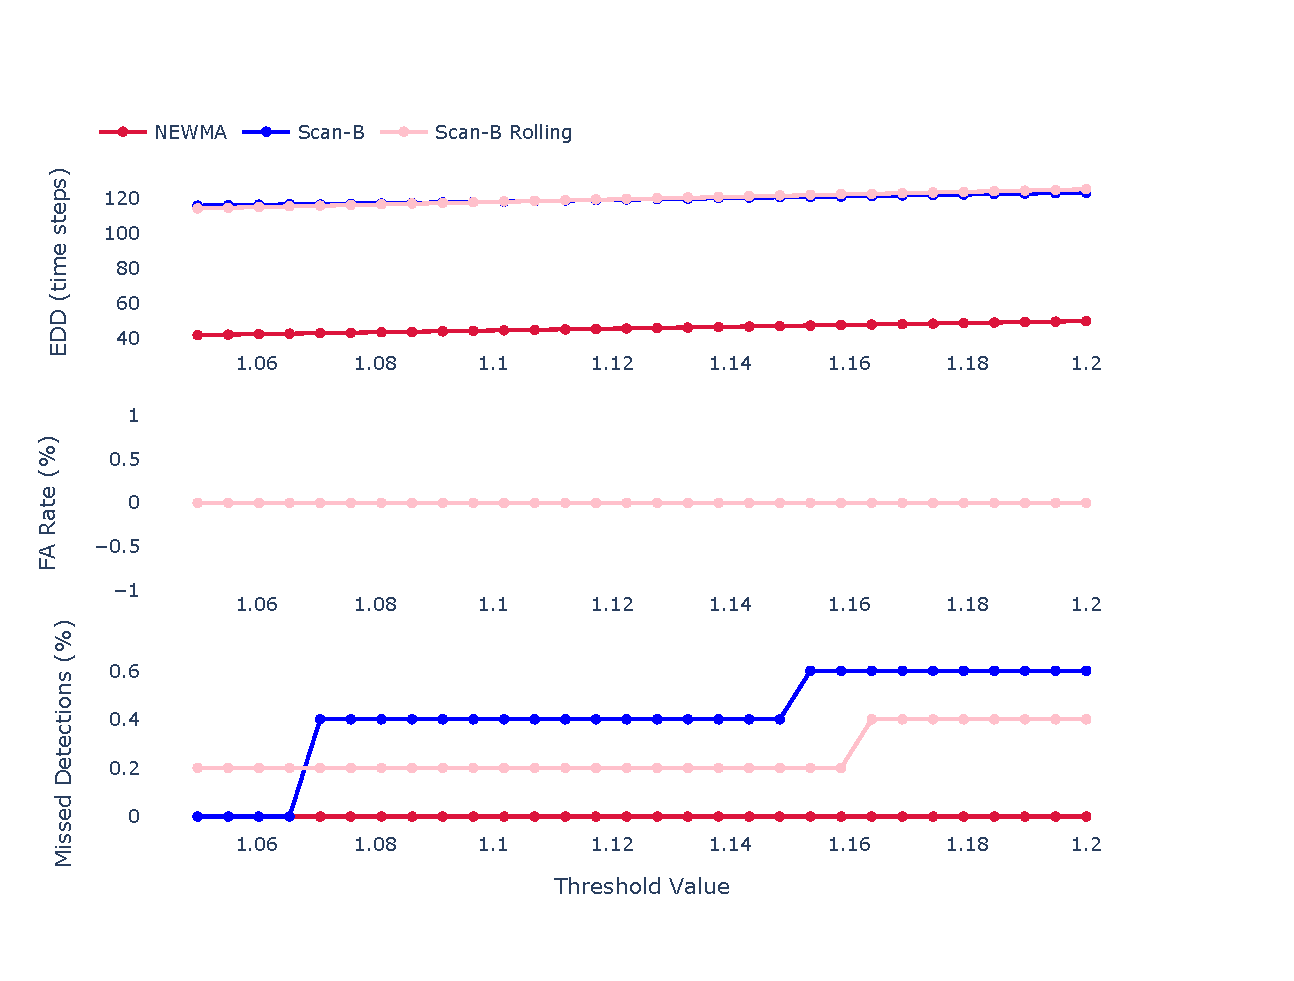
\includegraphics[trim=0cm 1cm 0cm 1cm, clip, width=\textwidth]{mean_shift} 
\label{fig:mean_shift_results} 
%\medskip
%\tiny
%(top) Daily stock prices (at closing) and (bottom) Daily returns on the stock (evaluated at closing) of Apple Inc. 
\end{center}
\end{minipage}

The results of the second variant of the mean shift occurring in a single dimension is shown figure \ref{fig:single_mean_results}. They tell the same story as the previous mean shift experiment, where again the two versions of Scan-B yields a similar performance in all respects, with slightly better missed detection rate at certain thresholds for the rolling median heuristic method. The NEWMA algorithm is again about three times lower EDD with no drawbacks in the other metrics.

\begin{minipage}{\textwidth}
\begin{center} 
\captionof{figure}[Evaluation Plots for change points of a Mean Shift in a Single Dimension]{Evaluation graphs for a mean shift in a single dimension, where expected detection delay (\textbf{top}), false alarm rate (\textbf{middle}), and missed detection rate (\textbf{bottom}) are plotted over a threshold region between $[1,1.2]$. } 
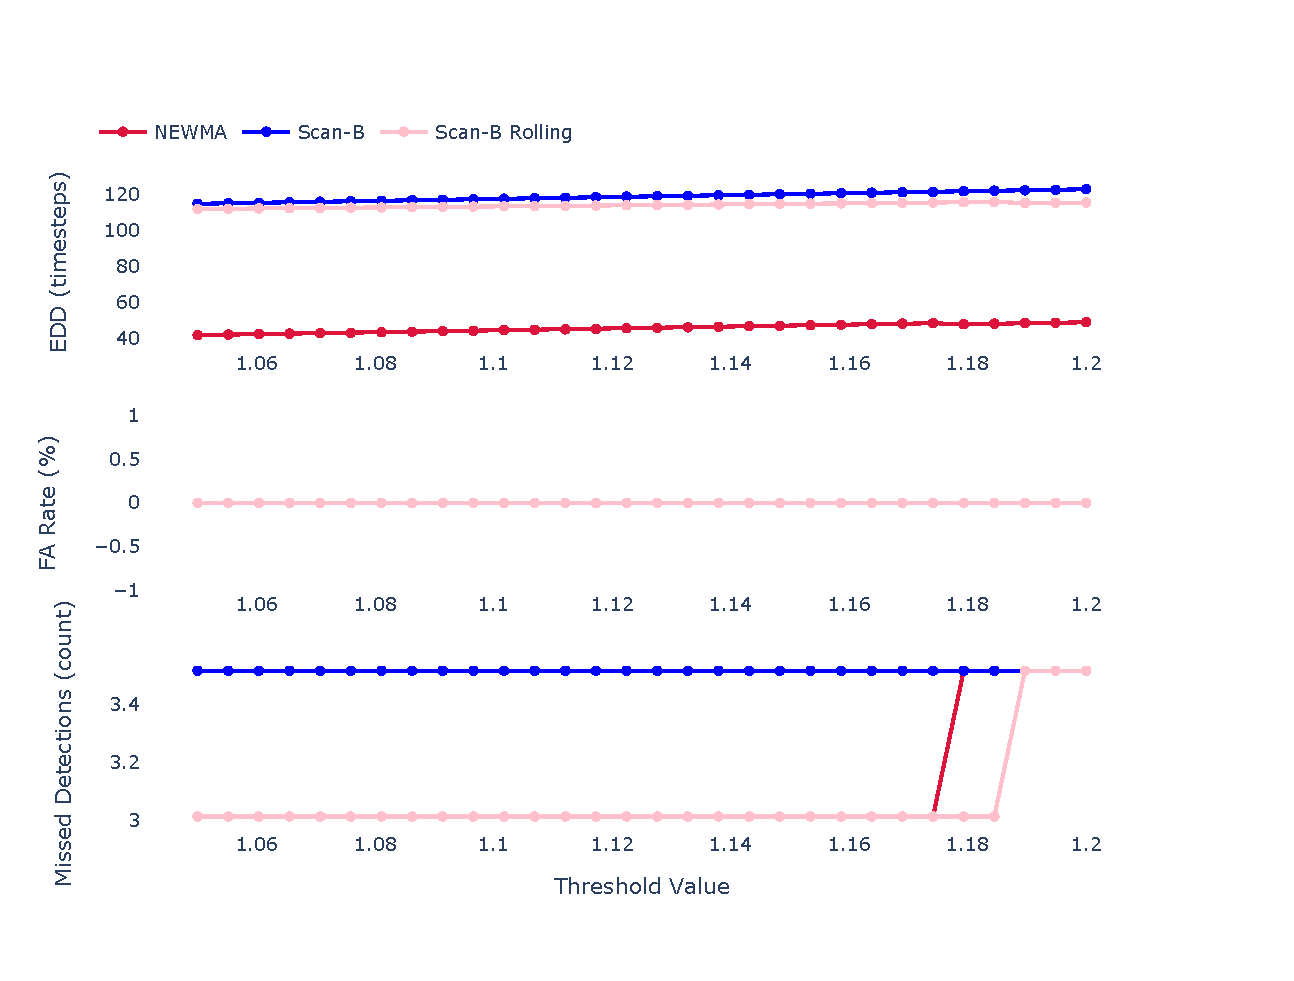
\includegraphics[trim=0cm 1cm 0cm 1cm, clip, width=\textwidth]{single_mean} 
\label{fig:single_mean_results} 
%\medskip
%\tiny
\end{center}
\end{minipage}

The worst performance of the rolling median heuristic version of Scan-B is presented in \ref{fig:variance_results}. The EDD is consistently worse across the different thresholds for the rolling Scan-B. While the false alarm rate is relatively still low, the algorithm missed many change points compared to NEWMA and the regular Scan-B algorithms, which did not miss any. This is a disappointing result because detecting changes in variance are a very common use case for change point detection models. Between NEWMA and regular Scan-B algorithms, both performed the same for missed detections and false alarms but NEWMA was considerably better in EDD with a more than $50\%$ improvement on average.

\begin{minipage}{\textwidth}
\begin{center} 
\captionof{figure}[Evaluation Plots for change points of a Variance Shift]{Evaluation graphs for a variance shift, where expected detection delay (\textbf{top}), false alarm rate (\textbf{middle}), and missed detection rate (\textbf{bottom}) are plotted over a threshold region between $[1,1.2]$. } 
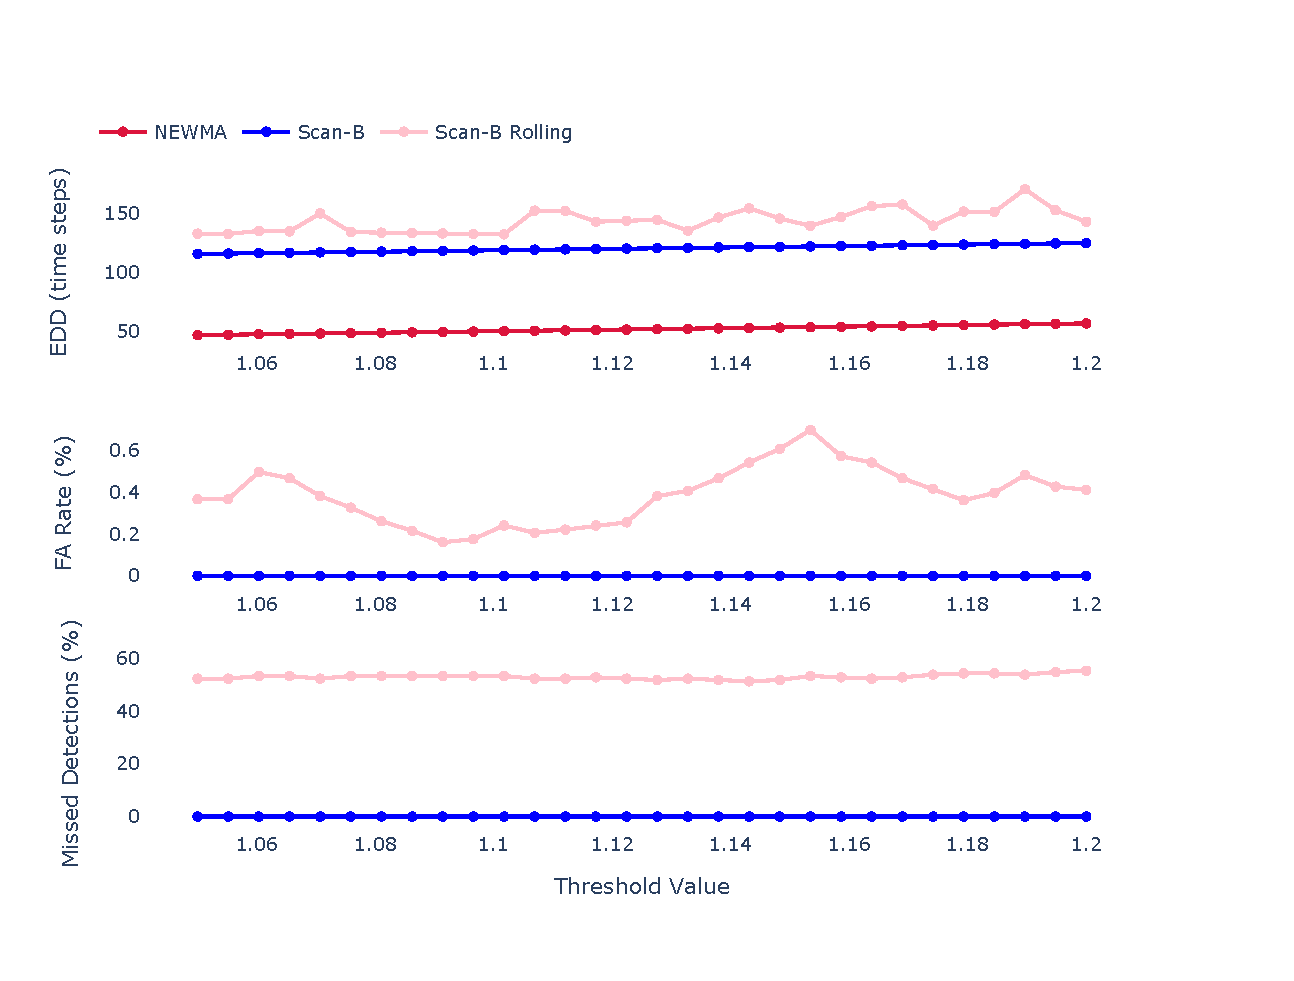
\includegraphics[trim=0cm 1cm 0cm 1cm, clip, width=\textwidth]{variance} 
\label{fig:variance_results} 
%\medskip
%\tiny
\end{center}
\end{minipage}

In the next experiment of alternating between GMMs with the results shown in figure \ref{fig:gmm_results}, the performance of the rolling median Scan-B is not as good overall to the standard counterpart. The EDD is consistently worse across thresholds and the missed detections rise up as well as the thresholds widen, leading to the conclusion that the algorithm is not sensitive enough in this situation to pick up the changes in distribution. It is simply rarely making any detections, hence why there are almost no false alarms, but many missed detections.

\begin{minipage}{\textwidth}
\begin{center} 
\captionof{figure}[Evaluation Plots for GMM change points]{Evaluation graphs for Gaussian mixture model change points, where expected detection delay (\textbf{top}), false alarm rate (\textbf{middle}), and missed detection rate (\textbf{bottom}) are plotted over a threshold region between $[1,1.2]$. } 
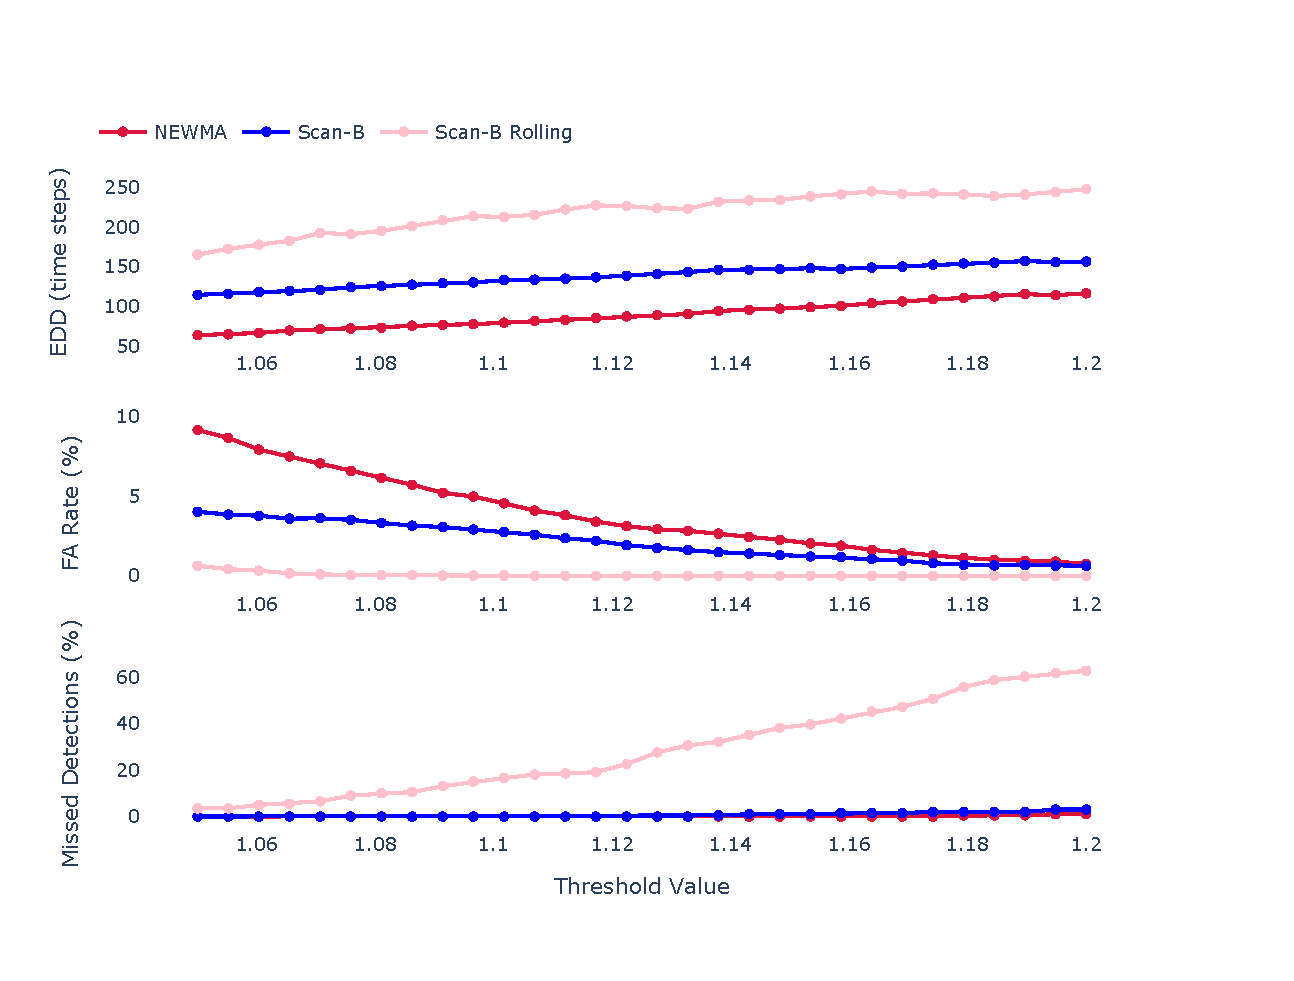
\includegraphics[trim=0cm 1cm 0cm 1cm, clip, width=\textwidth]{gmm} 
\label{fig:gmm_results} 
%\medskip
%\tiny
\end{center}
\end{minipage}

In figure \ref{fig:gauss_gmm_results}, the results are quite poor for the rolling median heuristic version of Scan-B. The false alarm rate is similar to the other kernel algorithms but the EDD and missed detections are considerably worse at various thresholds. The NEWMA algorithm and standard Scan-B are nearly identical across the board.

\begin{minipage}{\textwidth}
\begin{center} 
\captionof{figure}[Evaluation Plots for Gaussian to GMM change points]{Evaluation graphs for Gaussian to Gaussian mixture model change points, where expected detection delay (\textbf{top}), false alarm rate (\textbf{middle}), and missed detection rate (\textbf{bottom}) are plotted over a threshold region between $[1,1.2]$. } 
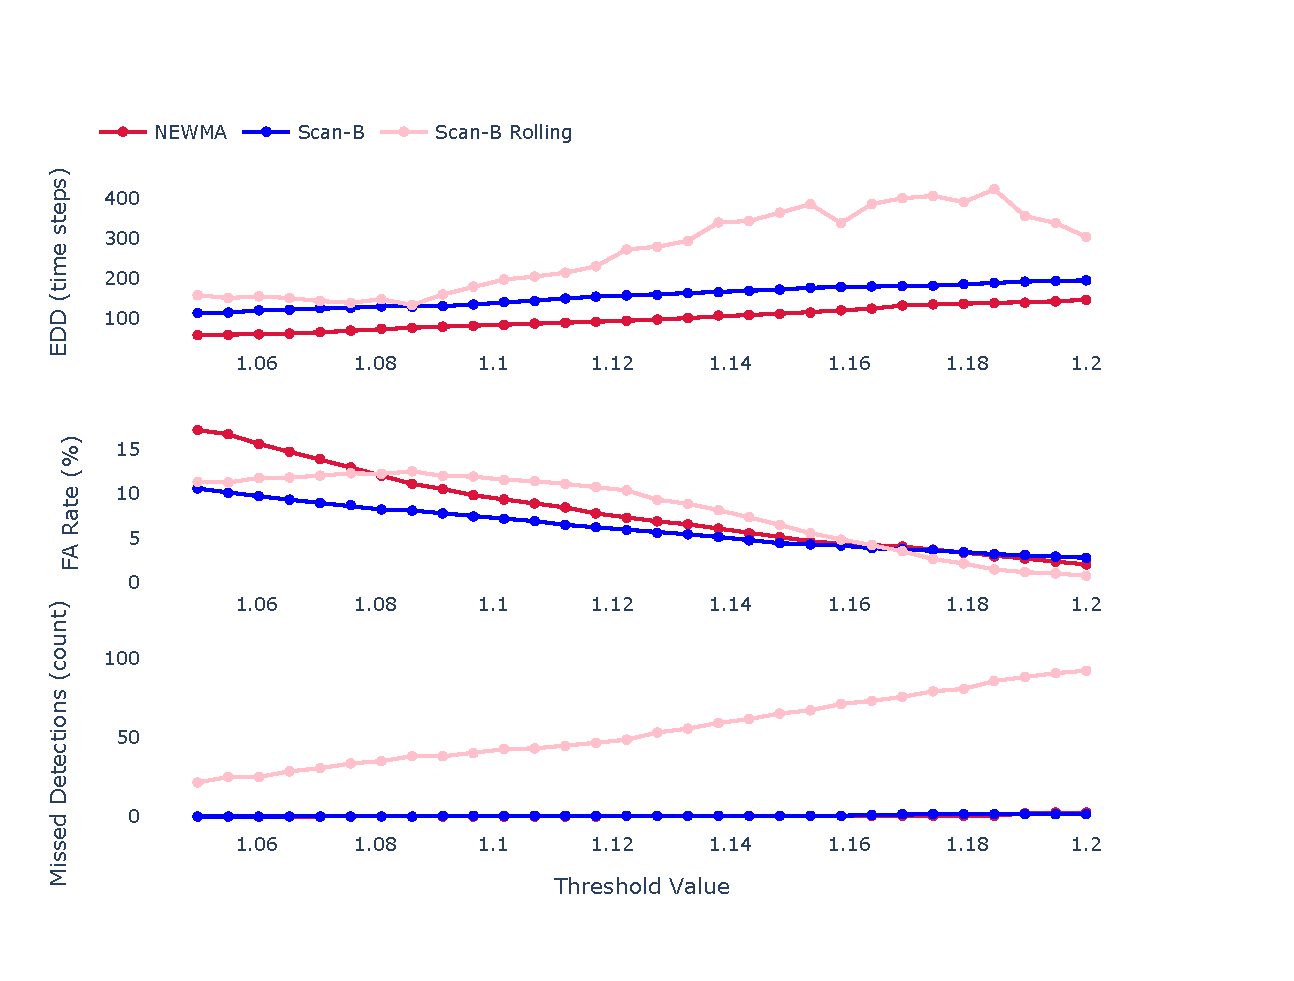
\includegraphics[trim=0cm 1cm 0cm 1cm, clip, width=\textwidth]{gauss_gmm} 
\label{fig:gauss_gmm_results} 
%\medskip
%\tiny
\end{center}
\end{minipage}

Finally as shown in \ref{fig:gauss_laplace_results}, the results of the Gaussian to Laplace change points demonstrate that the rolling median variation is tradeoff between the false alarm rate and the missed detections as it is equivalent to the other methods in terms of EDD. Regular Scan-B and NEWMA are quite similar for this experiment with very minor differences at a few thresholds.

\begin{minipage}{\textwidth}
\begin{center} 
\captionof{figure}[Evaluation Plots for Gaussian to Laplace change points]{Evaluation graphs for Gaussian to Laplace change points, where expected detection delay (\textbf{top}), false alarm rate (\textbf{middle}), and missed detection rate (\textbf{bottom}) are plotted over a threshold region between $[1,1.2]$. } 
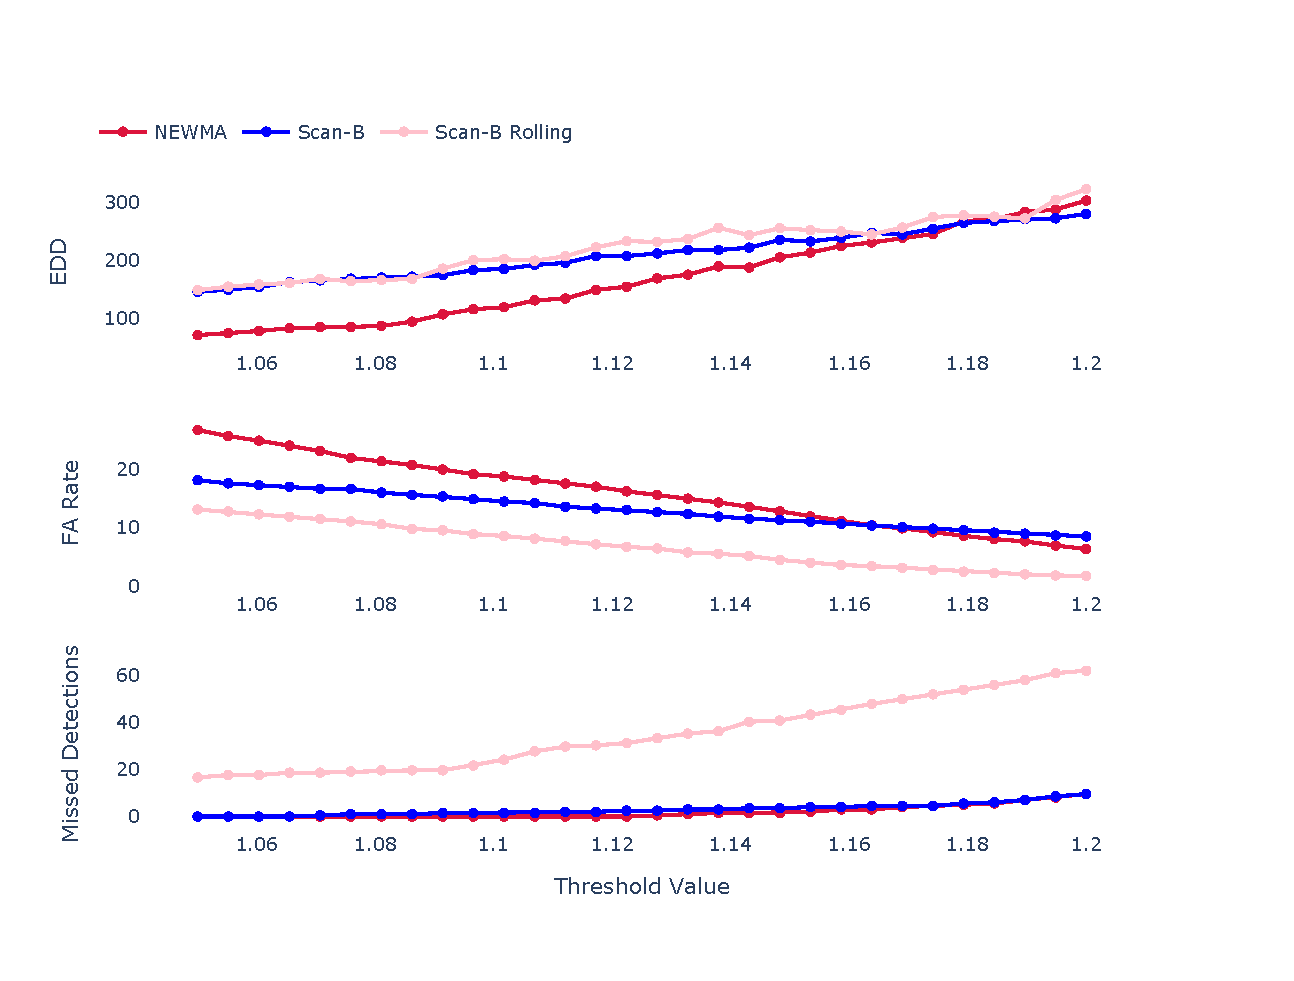
\includegraphics[trim=0cm 1cm 0cm 1cm, clip, width=\textwidth]{gauss_laplace} 
\label{fig:gauss_laplace_results} 
%\medskip
%\tiny
\end{center}
\end{minipage}

\subsection{Rolling Median Use Cases}

While the results of the previous section may seem like changing the median heuristic for the Gaussian kernel bandwidth to an online calculation, we present some particular use cases here where it is beneficial. Specifically, we setup some experiments that are particularly suitable for an online bandwidth estimation rather than a one-time estimation.

The first experiment involves a mean shift similar to the first experiment presented in the previous. However, in this case the mean shifts will be sequential in nature with an upward trend. That is the first distribution is a $d=20$ dimensional normal sampled from $\mathcal{N}(0,1)$. The second distribution increments the mean by $1$ yielding $\mathcal{N}(1,1)$. This pattern continues for $500$ change points until the final distribution is $\mathcal{N}(499,1)$. The results of the experiment are shown in figure \ref{fig:seq_mean_results}. As we can see the EDD is better for the rolling median bandwidth version of Scan-B by about $5-10\%$ over the range of thresholds. This improvement comes at no cost to the amount of false alarms or missed detections.

\begin{minipage}{\textwidth}
\begin{center} 
\captionof{figure}[Evaluation Plots for Incremental Mean Shift change points]{Evaluation graphs for incremental mean shift change points, where expected detection delay (\textbf{top}), false alarm rate (\textbf{middle}), and missed detection rate (\textbf{bottom}) are plotted over a threshold region between $[1,1.2]$. } 
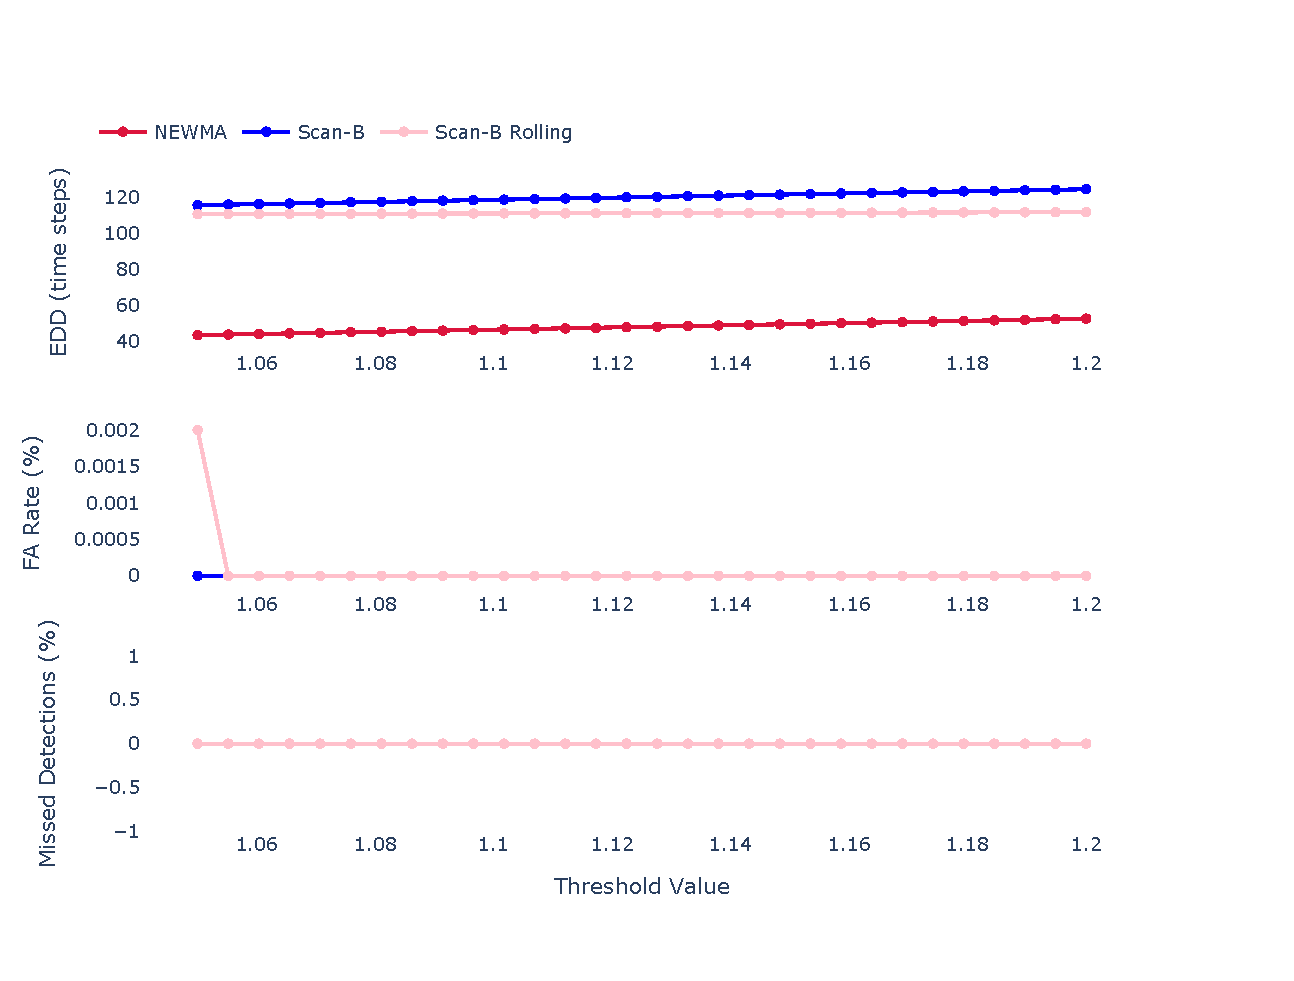
\includegraphics[trim=0cm 1cm 0cm 1cm, clip, width=\textwidth]{seq_mean_shift} 
\label{fig:seq_mean_results} 
%\medskip
%\tiny
\end{center}
\end{minipage}